\unchapter{Introduction}
\label{chap:introduction}
% \addcontentsline{toc}{chapter}{Introduction}
Notre peau est l’un des organes majeurs de notre corps ; ses lésions sont par conséquent nombreuses :  des plus anodines (communément appelées lésions bénignes), aux plus graves (dites lésions malignes) comprenant divers cancers aux répercussions les plus dramatiques.\par
La plupart des lésions malignes rencontrées sont d’origine cancéreuse, issues d’une division ou d’une mutation anormale de cellules de la peau et, résultent pour la plupart d’une exposition aux UV, principal facteur de risque.  D’autres facteurs tels que le tabagisme, les virus, des prédispositions génétiques ou encore l’utilisation de médicaments immunosuppresseurs (suite à une transplantation par exemple) favorisent leur apparition. Afin de limiter l’incidence de ces lésions, de nombreuses campagnes de prévention sont menées, intégrant sensibilisation et actions de prévention dans le but d’augmenter le confort de vie futur des individus, notamment au sein des pays les plus touchés.\par
Ces campagnes de sensibilisation à la prévention, bien que souvent sous des formes traditionnelles tel que des prospectus ou spots publicitaires, peuvent être de natures diverses. Nous pouvons citer à titre d’exemple, la mise en place de formations de prévention dès le plus jeune âge au sein des structures scolaires aux Etats Unis d’Amérique, ou à l’opposé la multiplication des supports de communication avec, par exemple, l’utilisation de sachets de sucres au Portugal \cite{Correia2017,Guy2016}.\par 
\begin{table}[H]
    \begin{tabular}{lll|lll}
    \textbf{Cancer}                     & \textbf{Incidence}& \textbf{Décès}& Prostate cancer                  & 1618               & 366           \\
    All cancers                         & 17481             & 8713          &  Testicular cancer               & 72                 & 9             \\
    Lip and oral cavity                 & 410               & 146           &  Kidney cancer                   & 425                & 137           \\
    Nasopharynx cancer                  & 123               & 63            &  Bladder cancer                  & 541                & 188           \\
    Other pharynx                       & 161               & 64            &  Système nerveux cancer          & 321                & 229           \\
    Esophageal cancer                   & 1313              & 891           &  Thyroid cancer                  & 334                & 32            \\
    Colon and rectum cancer             & 1653              & 832           &  Mesothelioma                    & 37                 & 32            \\
    Gallblader and biliary tract cancer & 188               & 140           &  Hodgkin lymphoma                & 78                 & 24            \\
    Pancreatic cancer                   & 426               & 412           &  Non Hodgkin lymphoma            & 666                & 231           \\
    Larynx cancer                       & 238               & 106           &  Multiple melyoma                & 154                & 101           \\
    Tracheal, bronchus and lung cancer  & 2019              & 1722          &  Leukemia                        & 606                & 353           \\
    Malignant skin melanoma             & 352               & 60            &  Acute lymphoid leukemia         & 161                & 110           \\
    Breast cancer                       & 2422              & 534           &  Chronic lymphoid leukemia       & 191                & 61            \\
    Cervical cancer                     & 526               & 239           &  Acute myeloid leukemia          & 190                & 147           \\
    Uterine cancer                      & 455               & 90            &  Chronic myeloid leukemia        & 64                 & 35            \\
    Ovarian cancer                      & 251               & 161           &  Other neoplasms                 & 756                & 372           \\
    \end{tabular}    
    \caption{Statistiques mondiales d’incidence et mortalité par type de cancers \cite{Karimkhani2017}.}
    \label{tab:cancer_incidence}
\end{table}\par
Néanmoins, ces actions tendent aujourd’hui à dépasser la prévention. En effet, certains articles essaient de montrer l’importance d’une auto surveillance régulière des individus au travers de gestes simples, dans le cadre de la détection de mélanome, permettant une prise en charge de la pathologie dans un meilleur délai.  Dans ce même objectif, nous pouvons également mentionner l’accroissement  du nombre de campagnes de dépistage mises en place par les gouvernements \cite{Friedman1985}.\par
Malgré ces démarches, le taux d’apparition de ces cancers ne cesse d’augmenter au travers des divers pays. De nos jours, le World Health Organization dénombre :
\begin{itemize}
\item entre 2 et 3 millions de cancers de la peau autre que le mélanome par an
\item environ 132,000 cancer de type mélanome par an.
\end{itemize}\par
D'un point de vue financier, les soins générés par les pathologies de la peau (toutes confondues) se chiffrent annuellement à 8 milliards de dollars aux Etats-Unis \cite{Farberg2017a}.\par

Pour la France, ce n’est pas moins de 5 100 nouveaux cas par an estimés de mélanome chez la femme et 4 680 chez l’homme, soit respectivement la 6ème et 8ème cause de cancer. Cette pathologie provoque environ 1 500 décès par an, genres confondus \cite{Thuret2012}.
Notre sujet « Aide au diagnostic/pronostic des lésions pigmentaires en dermatologie par analyse multi-échelle d’images multimodales » s’inscrit dans cette thématique, en tentant d’apporter des bases d’outils permettant d’aider le praticien dans sa prise de décision.\par
Cette thématique répond donc en premier lieu à un besoin sociétal, d’autant plus si nous constatons une baisse constante du nombre de dermatologues en France depuis 2010, visible en \Cref{fig:number_dermatologists}.
\begin{figure}[H]
    \centering
    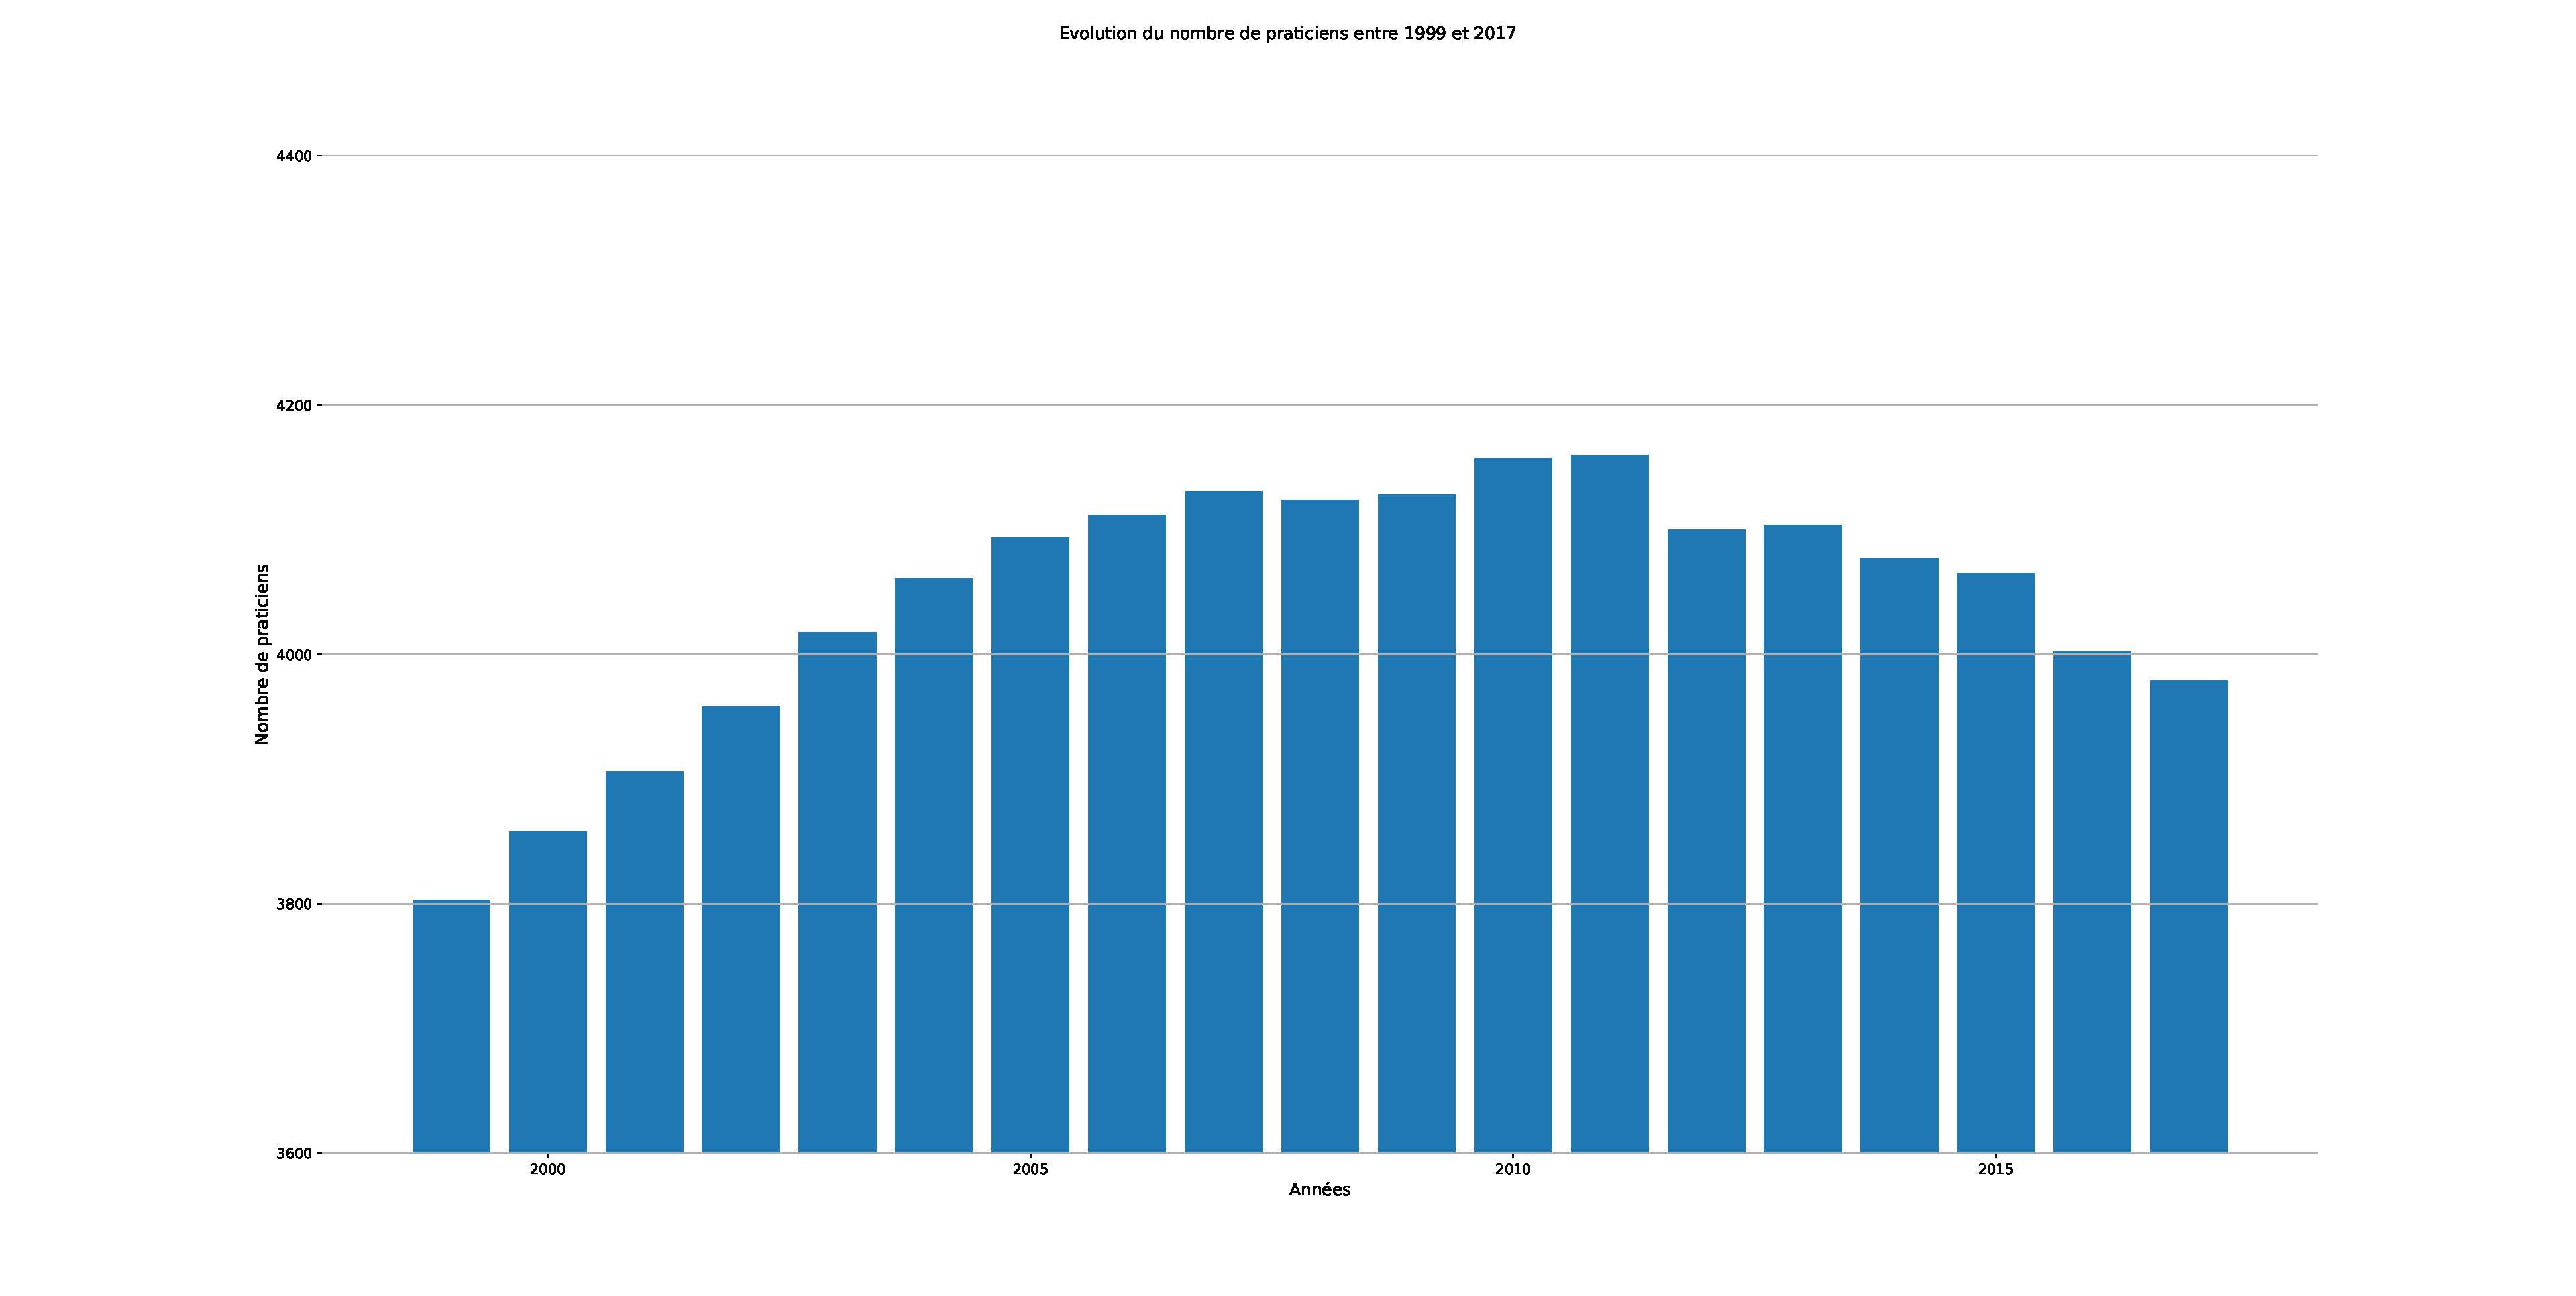
\includegraphics[width=\linewidth]{contents/x_introduction/resources/evolution_dermatologists.pdf}
    \caption{Evolution du nombre de dermatologues en France \textsuperscript{\ref{footnote:number_dermatologists}}.}
    \label{fig:number_dermatologists}
\end{figure}\par
\addtocounter{footnote}{1}
\footnotetext[\thefootnote]{Source image : Graphique généré à partir de données en provenance du site du  \href{http://www.data.drees.sante.gouv.fr/}{gouvernement} sur la santé. \label{footnote:number_dermatologists}}

Néanmoins, cette thématique ne demeure pas moins intéressante d’un point de vue scientifique. En effet, les 20 dernières années ont été portées par une forte tendance sur le sujet comme le démontre la \Cref{fig:evolution_publications}. Cette tendance est régie par plusieurs facteurs :
\begin{itemize}
\item Le besoin sociétal de la thématique, et l'intérêt porté par les industriels
\item Le phénomène "machine learning", et ses récentes avancées (notamment avec l'apprentissage profond)
\item Le "challenge" apporté par cette thématique, que nous développerons.
\end{itemize}\par
Ce sujet tentera d’apporter de nouveaux éléments de résolution, par l’apport notamment d’une dimension de multi modalité encore peu exploitée dans cette branche. 
\begin{figure}[H]
    \centering
    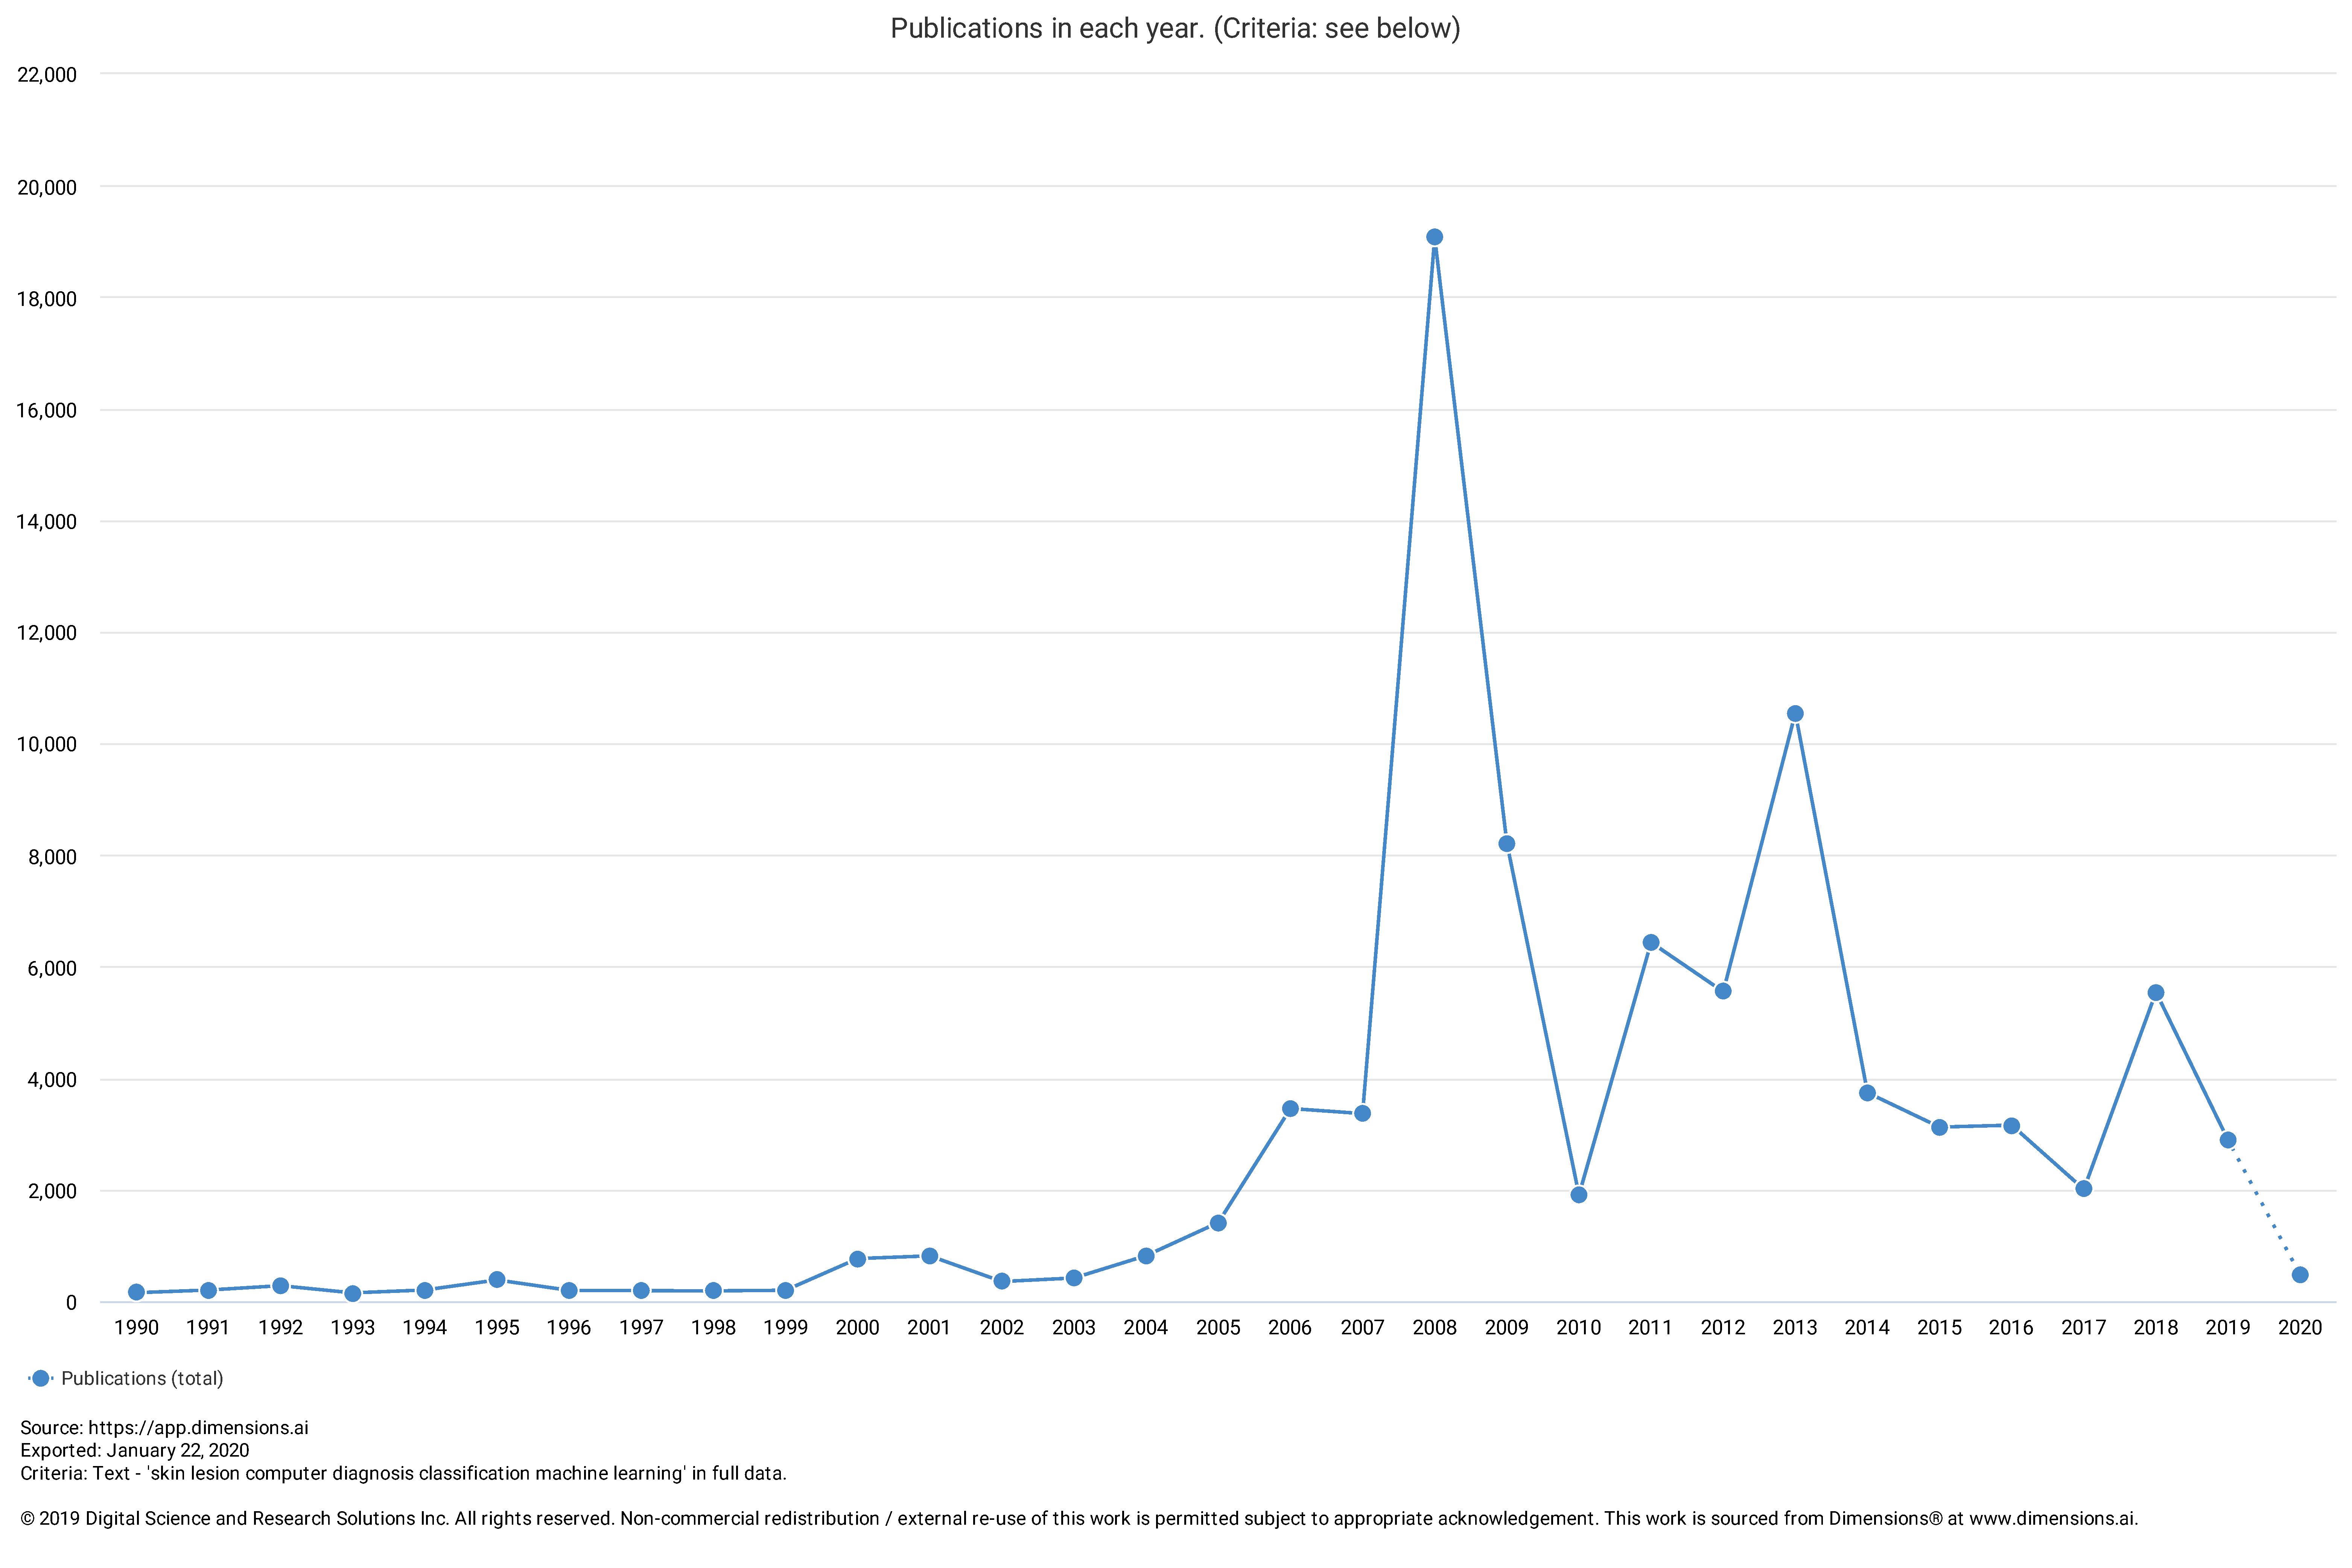
\includegraphics[width=\linewidth]{contents/x_introduction/resources/evolution_publications.pdf}
    \caption{Évolution de la recherche autour des termes "skin lesion computer diagnosis" durant ces 20 dernières années \textsuperscript{\ref{footnote:evolution_publications}}.}
    \label{fig:evolution_publications}
\end{figure}\par
\addtocounter{footnote}{1}
\footnotetext[\thefootnote]{Source image : Graphique généré à partir de données en provenance du moteur de recherche \href{https://scholar.google.fr/}{Google Scholar.} \label{footnote:evolution_publications}}
\clearpage